\chapter{Výsledky}
V této práci jsme studovali dvojice molekul $\mathrm{BeH/BeH^-}$ a $\mathrm{OH/OH^-}$, protože se jedná o dvouatomové molekuly s relativně nízkým počtem elektronů,
které mají vázaný jak základní stav, tak anion, a zároveň se jedná o 
dostatečně malé systémy, aby bylo možné provádět výpočty přesnými metodami.

Ke kvantově chemickým výpočtům jsme použili balík programů
MOLPRO\cite{MOLPRO-WIREs, MOLPRO}.
CAS-SCF výpočty jsme prováděli pomocí programu MULTI \cite{WK85,KW85}, MRCI výpočty 
pomocí programu CI \cite{KW92} a FCI výpočty pomocí programu FCI \cite{KH84,KH89}.

U referenčních výpočtů jsme pro několik desítek mezijaderných vzdálenost vypočítali 
energii základního stavu molekul pro fixovaná jádra. Ze znalosti těchto křivek jsme 
poté zjišťovali parametry molekul, které je 
možné nalézt experimentálně, což jsou disociační energie aniontu i neutrální molekuly 
a 
elektronové afinity molekuly  ve vázaném stavu i asymptotickou elektronovou afinitu, 
která odpovídá 
elektronové afinitě některého z prvků v molekule. Protože experimentální 
data nejsou určená minimem potenciální energie molekuly, ale základní vibrační 
hladinou, bylo třeba získat vibrační energetické hladiny dané molekuly metodou uvedenou 
v části \ref{te_vibr}. Počet geometrií, pro které jsme 
prováděli kvantově-chemické výpočty byl nedostatečný pro další numerické výpočty. Proto 
jsme získané hodnoty proložili kubickým splinem, ze kterého jsme
interpolovali hodnotu potenciálu v několika stovkách bodů. Poté jsme numericky získali 
energetické vibrační hladiny. Toto jsme opakovali pro různé volby báze a metody.

Při hledání popisu neutrální molekuly pro použití v R-maticových výpočtech jsme nejprve 
získali křivky stavů jdoucí 
k několika nejnižším asymptotám pomocí přesnější metody ve velké bázi, kterou jsme 
použili jako referenční. Poté jsme tytéž stavy získali metodou vhodnou pro R-maticový 
výpočet a srovnali. Křivky jsme vertikálně posunuli tak, aby byla 
totožná minima základního stavu u zkoumané metody a referenčního výpočtu.

\section{BeH}
Základní stav BeH je $^2\Sigma^+$ a asymptoticky pro velké mezijadené vzdálenosti jde k 
atomovým stavům $\mathrm{Be}(^1S) + \mathrm{H}(^2S)$. Základní stav $\mathrm{BeH}^-$ je 
$^1\Sigma^+$, který jde asymptoticky k $\mathrm{Be}(^1S) + \mathrm{H^-}(^1S)$.
Při disociaci aniontu záporný náboj zůstává na vodíku, protože berylium má 
zápornou elektronovou afinitu.

Asymptotické chování excitovaných stavů neutrální molekuly je v tabulce \ref{taBeHas}, 
kde je popsáno asymptotické chování pomocí atomových stavů, relativní energie asymptoty 
vůči nejnižší asymptotě a molekulové stavy jdoucí k dané asymptotě. V závorce 
je uvedena nejnižší asymptota, kterou jsme již ve výpočtech neuvažovali.

\begin{table}
\centering
\caption{Asymptotické chování stavů neutrální molekuly BeH pro velké mezijaderné 
vzdálenosti popsané atomovými stavy, energie vůči asymptotě základního stavu této 
molekuly a molekulové stavy jdoucí k této asymptotě.}
\bigskip
\label{taBeHas}
\begin{tabular}{ccc}
\toprule
asymptota & energie & molekulové stavy \\ 
\midrule
$\mathrm{Be}(^1\mathrm{S}) + \mathrm{H}(^2\mathrm{S})$ & $0.00$ & $^2\Sigma^+$ \\ 
$\mathrm{Be}(^3\mathrm{P}) + \mathrm{H}(^2\mathrm{S})$ & $2.725$ & $^2\Sigma^+,^4\Sigma^+,^2\Pi,^4\Pi$ \\
$\mathrm{Be}(^1\mathrm{P}) + \mathrm{H}(^2\mathrm{S})$ & $5.277$ & $^2\Sigma^+,^2\Pi$ \\ 
$\mathrm{Be}(^3\mathrm{S}) + \mathrm{H}(^2\mathrm{S})$ & $6.457$ & $^2\Sigma^+,^4\Sigma^+$ \\
$\mathrm{Be}(^1\mathrm{S}) + \mathrm{H}(^2\mathrm{S})$ & $6.779$ & $^2\Sigma^+$ \\
$\mathrm{Be}(^1\mathrm{D}) + \mathrm{H}(^2\mathrm{S})$ & $7.053$ & $^2\Sigma^+,^2\Pi,^2\Delta$ \\
$\left[\mathrm{Be}(^3\mathrm{P}) + \mathrm{H}(^2\mathrm{S})\right]$ &$[7.304]$& \\
\bottomrule
\end{tabular}
\end{table}


\subsection{Referenční výpočty}
Příklady křivek potenciální energie jsou vyobrazeny na obrázku  
\ref{VibrBeH1} spolu s vlnovými funkcemi základních vibračních hladin neutrální 
molekuly i aniontu.
Křivky v tomto obrázku byly získány metodou FCI v bázi aug-cc-pVTZ.

Pro srovnání s experimentem jsme provedli výpočty metodami FCI, CCSD(T) a MRCI jsme  
získali elektronovou afinitu molekuly v disociovaném i nedisociovaném 
stavu a disociační energie molekuly i jejího aniontu. Získané hodnoty jsou v tabulce \ref{beh1}. Pro každou metodu je pak za lomítkem 
uvedena použitá báze. Zkratka CBE označuje extrapolaci na úplnou bázi, z níž písmeny udáváme, které dvě aug-cc-pVXZ báze jsme použili pro výpočet dané hodnoty. U metody MRCI je navíc uveden použitý aktivní prostor
pro vstupní CAS-SCF výpočet,
zapsaný počtem jednotlivých molekulových orbitalů v dané ireducibilní reprezentaci v 
grupě $C_{2v}$ v pořadí $A_1, B_1, B_2, A_2$. 

Experimentální hodnotu disociační energie molekuly BeH jsme získali 
z \cite{BeH-LeRoy}, její elektronovou afinitu pak z \cite{BeH-ElAf}. Elektronová 
afinita atomárního vodíku je známa velmi přesně, 
najít lze například v \cite{H-ElAf}. Disociační energie aniontu jsme 
v literatuře nenalezli, ale
lze ji dopočítat pomocí
\begin{equation}
D_0(\mathrm{AB^-}) = D_0(\mathrm{AB}) + E_{a}(B) - E_{a}(AB), \label{eq_andiss}
\end{equation}
za předpokladu, že náboj zůstává na atomu B.V tomto vzorci značí $E_{a}$ elektronovou afinitu a $D_0$ disociační energii. Takto získanou hodnotu uvádíme v tabulce v závorce.
Nejnižší získané vibrační hladiny jsou v tabulce \ref{beh_vibr}.
Experimentální hodnoty jsme převzali z \cite{BeH-LeRoy}.
   
\begin{figure}
\centering
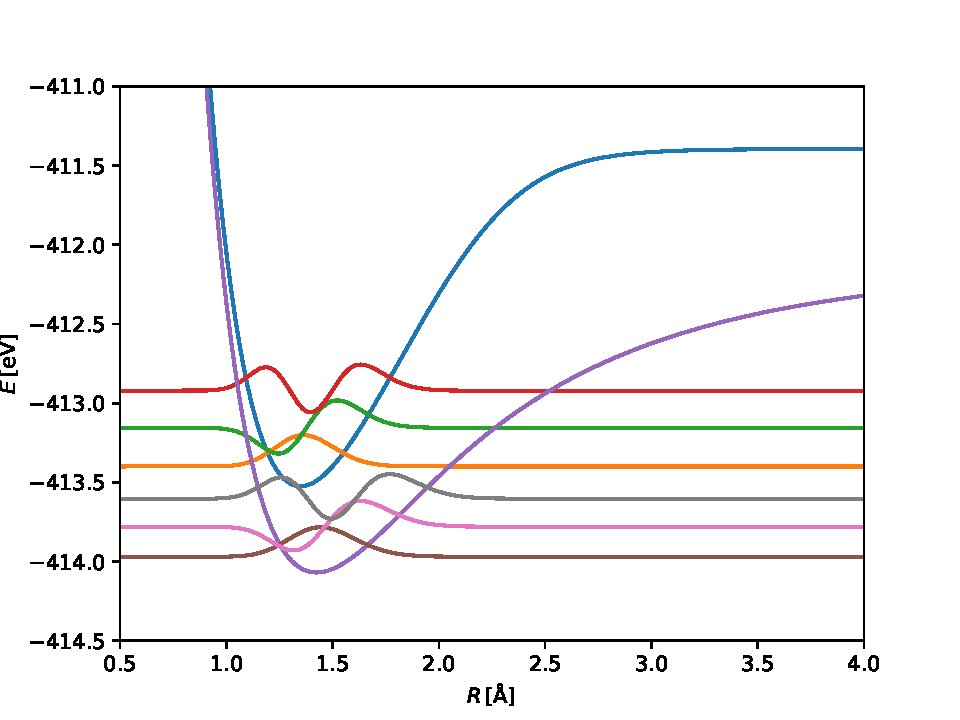
\includegraphics[width=0.95\textwidth]{../img/BeH-vibr1.pdf}
\caption{Potenciálové křivky základního stavu a nejnižší vibrační hladiny molekul $\mathrm{BeH/BeH^-}$}
\label{VibrBeH1}
\end{figure}
\htable{../tbl/BeH.tex}{Srovnání elektronové afinity molekuly BeH,elektronové afinity 
vodíku a disociačni energie BeH i $\mathrm{BeH^-}$ získaních více metodami v různých 
bázích s experimentem. Uváděné hodnoty jsou v elelektronvoltech.}{beh1}
\htable{../tbl/BeH-vibr.tex}{Nejnižší čtyři vibrační hladiny molekuly $\mathrm{BeH}$}{beh_vibr}
Z tabulky \ref{beh1} je vidět, že získaná asymptotická elektronová afinita závisí jen 
na použité bázi, a ve větší bázi se s metodou, případně aktivním prostorem vstupního 
CAS-SCF 
výpočtu pro MRCI mění jen nepatrně. Ostatní veličiny ovšem závisí i na velikosti báze, 
i na použité metodě, ale závislost na velikosti báze je o něco výraznější.
Z výpočtu metodou FCI v cc-pTVZ bázi je vidět,
že neaugmentované báze selhávají. To není 
překvapivé, je totiž všeobecně známo, že pro popis aniontů je třeba používat augmented 
báze.

Získaná elektronová afinita vodíku ve velkých bázích se blíží přesné 
hodnotě, ale jiné, především elektronová afinita, se výrazně liší od 
experimentu, navíc má evidentně tendenci konvergovat k jiné hodnotě, jak lze nahlédnout 
z extrapolací na úplnou bázi. Ovšem experiment udává poměrně velkou chybu měření (cca $14\%$),
navíc výpočty uvedené v \cite{Koput_BeH, Koput_BeHan} se s většinou experimentálních  
hodnot shodují, ale pro afinitu uvádí hodnotu $0.574\;\mathrm{eV}$, která je dosti 
vzdálená 
experimentální hodnotě, ale je v dobré shodě s našimi výsledky. Proto je třeba brát tuto hodnotu s rezervou, což by pak automaticky znamenalo, že nebude 
důvěryhodná ani udaná hodnota disociační energie aniontu získaná pomocí
\eqref{eq_andiss}. Nezanedbatelný je i rozdíl mezi našimi výpočty a experimentem v 
disociační energii neutrální molekuly, ale u té se ve výše zmíněném článku 
\cite{Koput_BeH} autorům podařilo dosáhnout hodnoty v rozmezí experimentální chyby.
Museli ovšem použít větší bázi,  
metodu, která je size konzistentní a provést relativistickou korekci i korekci na 
Bornovu-Oppenheimerovu aproximaci. 

Na druhou stranu, pro použití v R-maticových výpočtech je třeba, aby metoda dávala   
především pro všechny geometrie dostatečně přesný rozdíl energie neutrální molekuly a 
aniontu. Proto jsme odečetli energie potenciálových křivek neutrální molekuly BeH a jejího aniontu
získaných několika metodami v různých bázích a získali křivky v grafu \ref{grBeHlin}.
V popisku je uvedena jen metoda, různé čáry stejné barvy odpovídají různým použitým bázím.
Z něj je vidět, že relativní rozdíly mezi metodami i bázemi jsou nepatrné. Proto jsme
vzali křivku získanou metodou MRCI s aktivním prostorem vstupního CAS-SCF 6,2,2,0 v 
aug-cc-pV5Z bázi, kterou jsme odečetli od ostatních křivek. Požili jsme jednak křivky 
získané stejnou metodu v několika menších bázích a pro srovnání MRCI s aktivním 
prostorem 5,1,1,0 ve stejné bázi jako referenční výpočet a FCI v aug-cc-pVTZ bázi.
výsledky jsou v grafu \ref{grBeHlindif}. Z něj lze usuzovat, že pro dostatečně velkou 
bázi jsou rozdíly mezi metodami malé, a tedy je pro referenční výpočet třeba 
použít metodu MRCI v dostatečně velké bázi. Vzhledem k tomu, že v aug-cc-pVTZ bázi je 
křivka MRCI s aktivním prostorem 6,2,2,0 pro vstupní CAS-SCF výpočet velmi blízko FCI, 
lze očekávat, že je tento aktivní prostor rozumně zvolen. Proto se jako dobrý kandidáa 
kandidát na referenční výpočty pro nastavení výpočtu R.matic jeví výpočet MRCI s aktivním 
prostorem vstupního CAS-SCF 6,2,2,0 v aug-cc-pV5Z, případně
extrapolovaný na úplnou bázi.

\begin{figure}
\centering
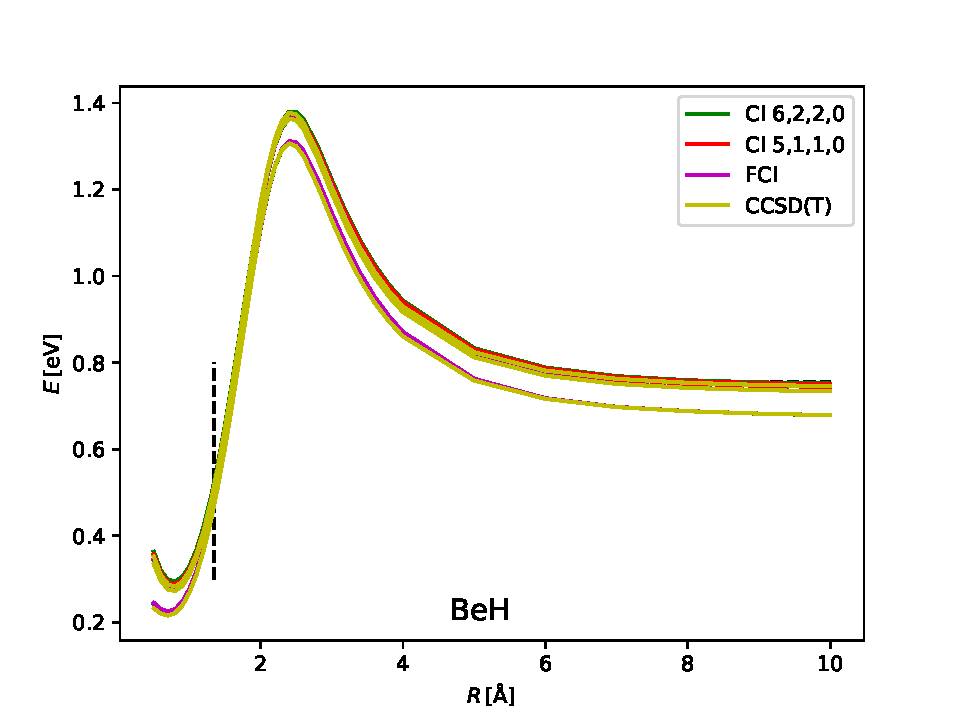
\includegraphics[width=0.95\textwidth]{../img/BeH-lin.pdf}
\caption{Vertikální elektronová afinita pro různě mezijaderné vzdálenosti, vodorovná čárkovaná čára označuje správné asymptotické chování, svislá pak rovnovážnou vzdálenost neutrální molekuly. Jedné metodě v legendě odpovídá více čar v různých bázích.}
\label{grBeHlin}
\end{figure}

\begin{figure}
\centering
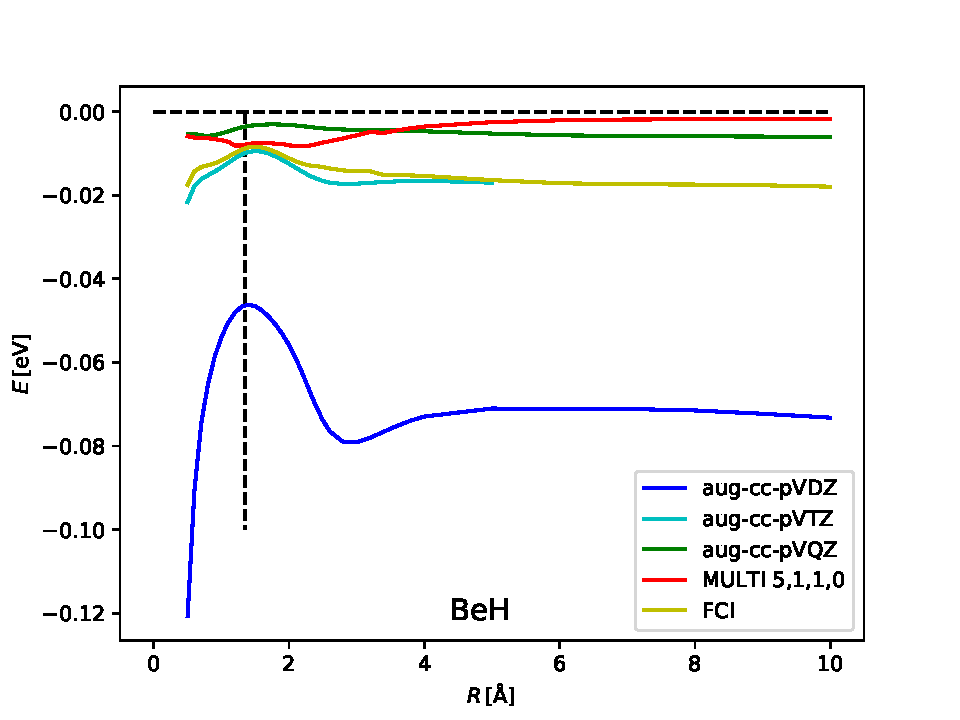
\includegraphics[width=0.95\textwidth]{../img/BeH-lin-dif.pdf}
\caption{Rozdíl křivek zobrazených v grafu \ref{grBeHlin}. Jako referenční metodu jsme použili MRCI 6,2,2,0 v aug-cc-pV5Z bázi,kterou jsme odečetli od ostatních metod.
Křivky v legendě označené názvem báze jsou získány pomocí MRCI 6,2,2,0 v dané bázi, FCI, je pak v aug-cc-pVTZ bázi a MRCI 5,1,1,0 je aug-cc-pV5Z bázi.}
\label{grBeHlindif}
\end{figure}

Vibrační hladiny se blíží hodnotám z experimentu. Z tabulky \ref{beh_vibr} je 
vidět, že pro jejich přesnost je podstatnější použitá báze než samotná metoda, s 
výjimkou metody CCSD(T), která dává vyšší energie hladin než ostatní metody v dané 
bázi, protože má obecně tendenci zužovat potenciálovou jámu oproti přesnému tvaru.

Nejlépe z výpočtů vibračních hladin sice vychází metoda CCSD(T) v aug-cc-pVQZ bázi, která ovšem špatně popisuje
molekuly pro mezijaderné vzdálenosti v přechodu mezi rovnováhou a asymptotou.
To je pro naší aplikaci podstatné, a proto se tato metoda pro referenční výpočet příliš 
nehodí. Navíc shoda s experimentem je pravděpodobně způsobena náhodným vyrušením chyby způsobené metodou a chyby způsobené bází.

\subsection{Popis targetu}
Ačkoliv lze pro takto malý systém použít metodu FCI se zamrznutým nejnižším molekulovým 
orbitalem, jak lze najít například v \cite{BeH-Rmat}, jedná se o časově náročný 
výpočet. Proto jsme se pokusili najít metodu CAS-SCF s takovými parametry, aby 
dostatečně dobře reprodukovala hodnoty získané přesnějšími metodami, protože by výrazně 
zkrátila R-maticový výpočet.
Prvně jsme provedli výpočet metodou FCI s 1 zamrznutým orbitalem v bázi aug-cc-pVTZ, 
který jsme použili jako referenční. Tentýž výpočet jsme provedli i s bází aug-cc-pVDZ, 
přičemž srovnání je na obrázku \ref{gr_Beh_FCI}. Z něj vidíme, že od stavů s rozdílem 
od základního stavu vyšším než cca 6 eV selhává popis pomocí aug-cc-pVDZ báze, a tedy 
přesnost metod nad touto úrovní nemá smysl uvažovat, neboť větší báze již nelze v R-
maticových výpočtech použít kvůli výpočetní náročnosti. Je vidět, že i metoda FCI se na 
některých místech chová špatně, především kvůli velkému množství blízkých stavů, 
přičemž se nám nedařilo zvolit počet stavů tak, aby nějaký vyšší, který jsme již 
neuvažovali, nezasahoval do již zvolených stavů. U metody FCI to nedělalo tak výrazné 
potíže s výjimkou některých zlomů a přeskakování ve vyšších excitovaných stavech, ale  
nepodařilo se nám kvůli tomu provést výpočet metodou MRCI, 
který by uvažoval takovéto množství excitovaných stavů.

Zkusili jsme srovnat několik metod CAS-SCF v aug-cc-pVDZ bázi lišících se aktivním 
prostorem a zjistili, že v okolí rovnovážné vzdálenosti dobře popisuje molekulu CAS-SCF 
v této bázi s 
aktivním prostorem $6,2,2,0$, které je zobrazeno na obrázku \ref{gr_Beh_6220} spolu s 
referenčním FCI v aug-cc-pVTZ bázi na pozadí šedou barvou. Zvětšení aktivního prostoru 
vedlo k zhoršení 
konvergence metody, čímž vzniklo v křivkách velké množství nespojitostí. To by 
teoreticky bylo možné odstranit nalezením vhodných vah pro jednotlivé stavy, ale popis 
by pravděpodobně nebyl o tolik lepší. Bez zadaných vah je výpočet s aktivním prostorem 
8,3,3,0 na obrázku \ref{gr_Beh_8330}.
Dobrá konvergence aktivního prostoru 6,2,2,0 je dána tím, že se jedná o úplný valenční 
prostor této molekuly - tedy prostor molekulových orbitalů, které vzniknou kombinací 
atomových orbitalů uzavřených a valenčních slupek obou atomů.

Ve všech výpočtech jsme 
nechali zamrznutý nejnižší molekulový orbital, ale jeho nezamrznutí téměř nemělo vliv 
na výsledek, což jsme pozorovali u zmíněného CAS-SCF výpočtu s aktivním prostorem 6,2,2,0.

V okolí rovnovážné geometrie první zmíněná metoda CAS-SCF popisuje velmi dobře křivky 
získané metodou FCI pro stavy s energií do 6 eV nad základním stavem, kde začíná 
selhávat použitá báze. Pro větší mezijaderné vzdálenosti pak metoda nedává dobré 
výsledky, ale to je obecný problém CAS-SCF metod a v R-maticových výpočtech nedělá 
tento jev až tak velké potíže.

Pro srovnání jsme provedli CAS-SCF výpočet s aktivním prostorem 6,2,2,0 v cc-PVTZ bázi, 
který popisuje molekulu mnohem hůř a je v grafu \ref{gr_Beh_TZ}. Je tedy 
pravděpodobné, že pro tuto molekulu je nutné použít augmented bázi.
\begin{figure}
\centering
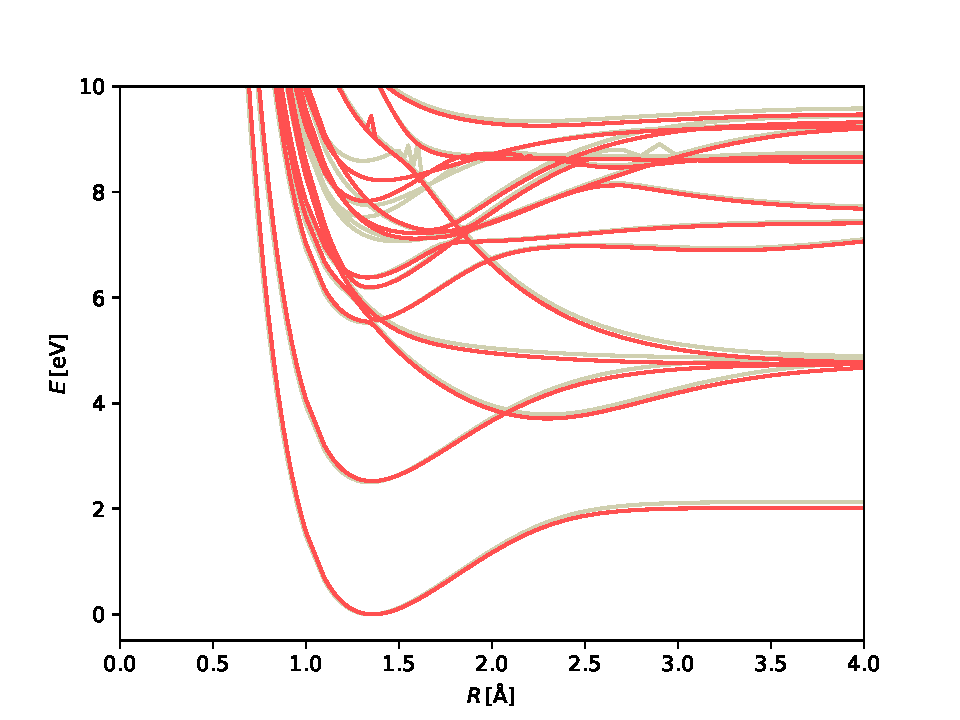
\includegraphics[width=0.95\textwidth]{../img/BeH-FCI-DZ.pdf}
\caption{Srovnání metody FCI pro neutrální molekulu BeH v bázi aug-cc-pVDZ (červená) a referenčním FCI v bázi aug-cc-pVTZ (šedá)}
\label{gr_Beh_FCI}
\end{figure}

\begin{figure}
\centering
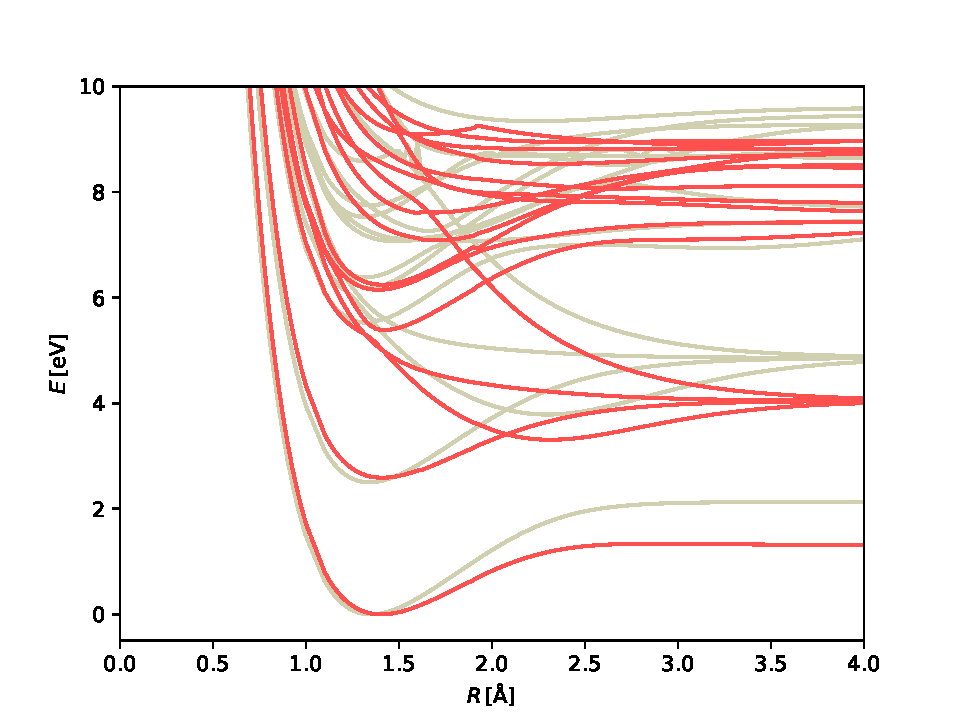
\includegraphics[width=0.95\textwidth]{../img/BeH-MULTI-DZ-6220.pdf}
\caption{Srovnání CAS-SCF výpočtu s aktivním prostorem $6,2,2,0$ v aug-cc-pVDZ bázi s referenčním FCI}
\label{gr_Beh_6220}
\end{figure}

\begin{figure}
\centering
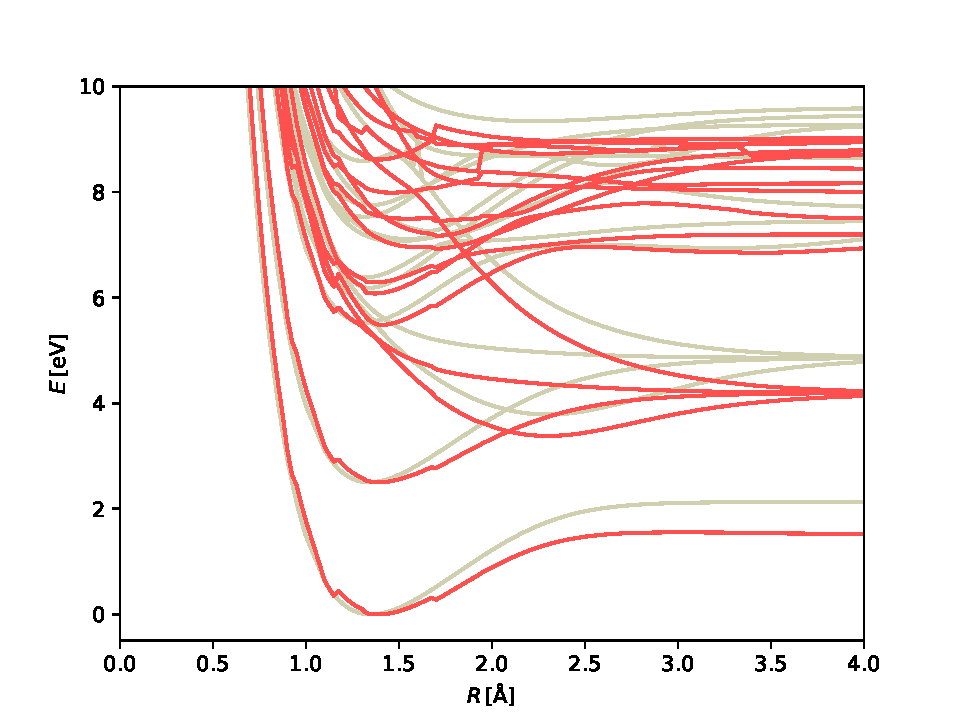
\includegraphics[width=0.95\textwidth]{../img/BeH-MULTI-DZ-8330.pdf}
\caption{Srovnání CAS-SCF výpočtu s aktivním prostorem $8,3,3,0$ v aug-cc-pVDZ bázi s referenčním FCI}
\label{gr_Beh_8330}
\end{figure}

\begin{figure}
\centering
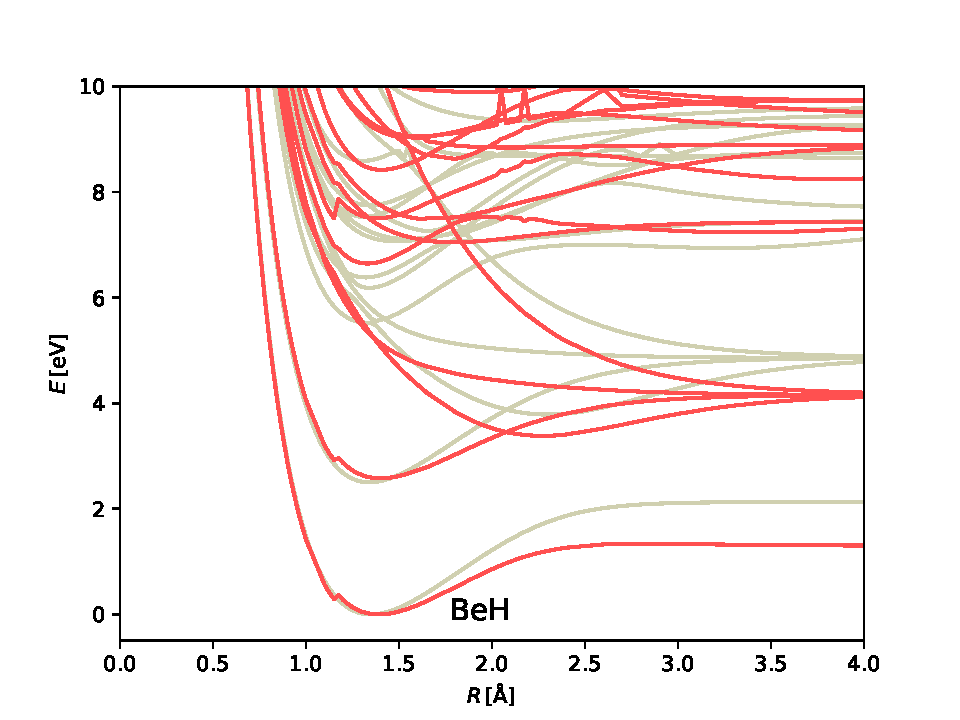
\includegraphics[width=0.95\textwidth]{../img/BeH-MULTI-TZ-6220.pdf}
\caption{Srovnání CAS-SCF výpočtu s aktivním prostorem $6,2,2,0$ v cc-pVTZ bázi s referenčním FCI}
\label{gr_Beh_TZ}
\end{figure}


\section{OH}
Základní stav molekuly OH je $\mathrm{^2\Pi}$ s asymptotou 
$\mathrm{O}(^3P) + \mathrm{H}(^2S)$. Další 
stavy jdoucí k této asymptotě jsou $\mathrm{^4\Pi, ^4\Sigma^-, ^2\Sigma^- }$.
Nejnižší tři asymptoty neutrální molekuly jsou pak v tabulce \ref{taOHas}, v závorce je
první asymptota, kterou jsme neuvažovali.

 Anion $\mathrm{O`^-}$ je v základním stavu $^1\Sigma^+$ s asymptotou
  $\mathrm{O^-}(^2\mathrm{P}) + \mathrm{H}(^2\mathrm{S})$. 
  K této asymptotě jdou ještě stavy
  $\mathrm{^3\Sigma^+,^1\Pi, ^3\Pi}$.
 Pod asymptotou základního stavu neutrální molekuly leží i asymptota 
 $\mathrm{O}(^3\mathrm{P}) + \mathrm{H^-}(^1\mathrm{S})$, 
 ke které jdou stavy $\mathrm{^3\Sigma^-, ^3\Pi}$.

\begin{table}
\centering
\caption{Asymptotické chování nejnižších stavů neutrální molekuly OH}
\label{taOHas}
\bigskip
\begin{tabular}{ccc}
\toprule
asymptota & energie asympt. & molekulové stavy \\ 
\midrule
$\mathrm{O}(^3\mathrm{P}) + \mathrm{H}(^2\mathrm{S})$ & $0.000$ & $\mathrm{^2\Sigma^-}, \mathrm{^4\Sigma^-},\mathrm{^2\Pi},\mathrm{^4\Pi}$ \\ 
$\mathrm{O}(^1\mathrm{D}) + \mathrm{H}(^2\mathrm{S})$ & $1.967$ & $\mathrm{^2\Sigma^+}, \mathrm{^2\Pi}, \mathrm{^2\Delta}$ \\ 
$\mathrm{O}(^1\mathrm{S}) + \mathrm{H}(^2\mathrm{S})$ & $4.190$ & $ \mathrm{^2\Sigma^+}$ \\ 
$[\mathrm{O}(^5\mathrm{S}) + \mathrm{H}(^2\mathrm{S})]$ & $[9.146]$ \\ 
\bottomrule
\end{tabular} 
\end{table}

Ukázka křivek pro všechny uvažované stavy neutrální molekuly i aniontu jsou vyobrazeny v grafu \ref{grOHL}. Křivky byly získány metodou MRCI s aktivním prostorem pro vstupní CAS-SCF výpočet 8,2,2,0 v aug-cc-pVQZ bázi.


\begin{figure}
\centering
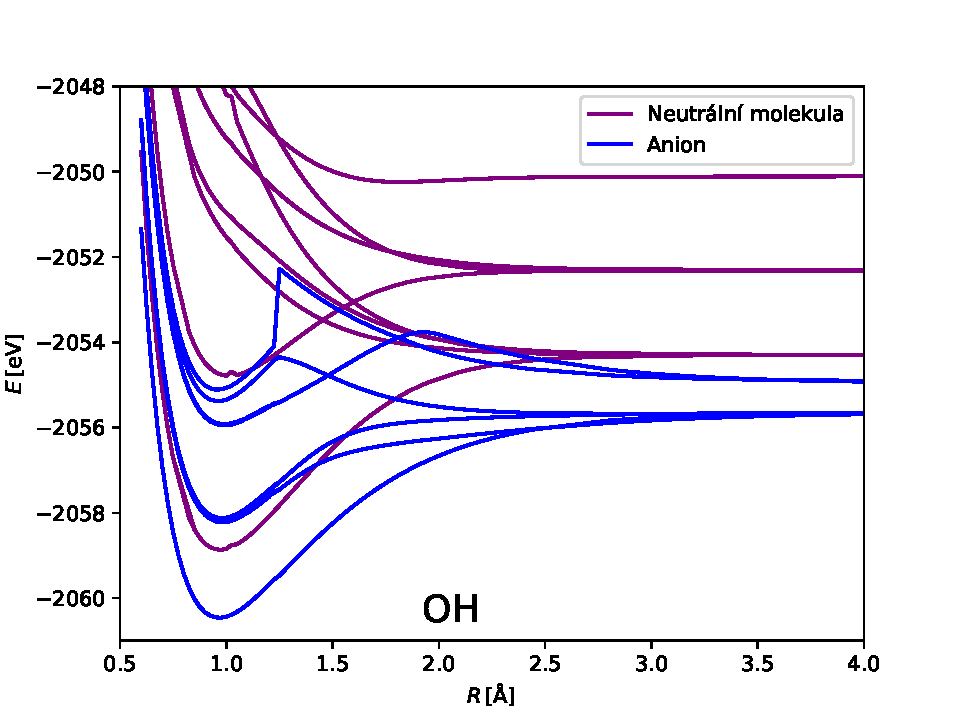
\includegraphics[width=0.95\textwidth]{../img/OHstates.pdf}
\caption{Potenciálové křivky stavů neutrální molekuly OH jdoucích ke 3 nejnižším asymptotám a aniontu $\mathrm{OH^-}$. U křivek aniontu v místech, kde zasahují nad křivku základního stavu neutrální molekuly již elektron není vázaný, a tedy získaná křivka v této oblasti již je nefyzikální.}
\label{grOHL}
\end{figure}

\subsection{Referenční výpočty}
Pro různé metody jsme získali křivky základního stavu neutrální molekuly i aniontu. 
Jiné křivky aniontu ani nejnižší asymptoty neutrální molekuly jsme neuvažovali, protože 
nejsou vázané a jedinou jejich veličinou srovnatelnou s experimentem je jejich 
asymptotické chování. To se pak navíc dá nastavit posunutím křivky a běžně se to při 
použití křivek v R-maticových výpočtech provádí.
Z nich jsme získali
disociační energii energie aniontu i neutrální molekuly, i rovnovážnou a asymptotickou 
elektronovou afinitu neutrální molekuly. Získané hodnoty, spolu s experimentálními daty 
jsou v tabulce \ref{oh1}
Hodnotu disociační energie neutrální molekuly uvádí například \cite{CRC_Handbook90}, 
stejně jako elektronovou afinitu této molekuly i atomárního kyslíku. Disociační energii 
aniontu jsme získali stejně jako u molekuly BeH pomocí \ref{eq_andiss}.

\begin{figure}
\centering
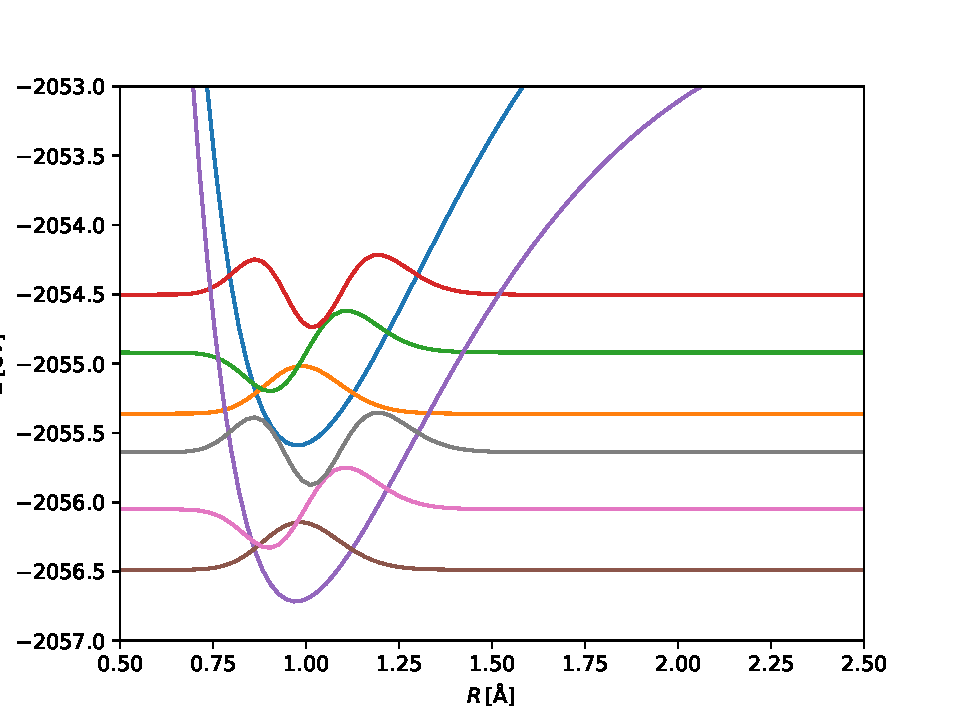
\includegraphics[width=0.95\textwidth]{../img/OH-vibr1.pdf}
\caption{Potenciálové křivky základního stavu a nejnižší vibrační hladiny molekul $\mathrm{OH/OH^-}$ \label{VibrOH1}}
\end{figure}

\htable{../tbl/OH.tex}{Srovnání elektronové afinity molekuly OH,elektronové afinity 
vodíku a disociační energie OH i $\mathrm{OH^-}$ získaných několika metodami v různých 
bázích s experimentem. Uváděné hodnoty jsou v elelektronvoltech. Poslední řádek odpovídá křivkám posunutým tak, aby elektronová afinita molekuly odpovídala experimentu.}{oh1}


Je vidět, že všechny zmíněné veličiny se se zvětšující bází přibližují experimentálním 
hodnotám. Při extrapolaci na úplnou bázi metody MRCI s aktivním prostorem 6,2,2,0 
dokážeme dosáhnout experimentální hodnoty disociační energie neutrální molekuly i 
očekávané disociační energie aniontu. Elektronové afinity molekuly ani asymptoty 
nedokážeme dosáhnout ani při extrapolaci na úplnou bázi, ale jejich rozdíl je téměř 
totožný. Tedy vertikální posunutím křivek tak, aby disociační energie molekuly 
odpovídala experimentu, dokážeme získat téměř přesnou hodnotu asymptotické energie. 
 
V grafu \ref{grOHlin} je pak rozdíl potenciálových křivek neutrální molekuly OH a 
aniontu, získaných metodami MRCI 6,2,2,0 a MRCI 8,2,2,0 v různých bázích. Z něj je 
vidět, že asymptotické chování se blíží přesnému jen velmi pomalu se 
zvětšující se bází a téměř vůbec s větším aktivním prostorem CAS-SCF výpočtu.
V grafu \ref{grOHlindif} jsou pak relativní rozdíly křivek v grafu \ref{grBeHlin} vůči 
křivce získané pomocí MRCI 8,2,2,0 v aug-cc-pV5Z bázi. Z tohoto grafu je vidět, že pro 
zvětšující bázi se křivky získané stejnou metodou mění čím dál víc ě lineárně. 
Proto je možno očekávat, že pokud posuneme křivky aby byla správná elektronová 
afinita vázaného stavu i asymptoty, rozdíl ve všech bodech bude blízko přesné 
hodnoty. Navíc i rozdíly mezi MRCI 6,2,2,0 a MRCI 8,2,2,0 ve stejné bázi
 jsou ve všech bodech křivek do cca 0.015 eV.

\begin{figure}
\centering
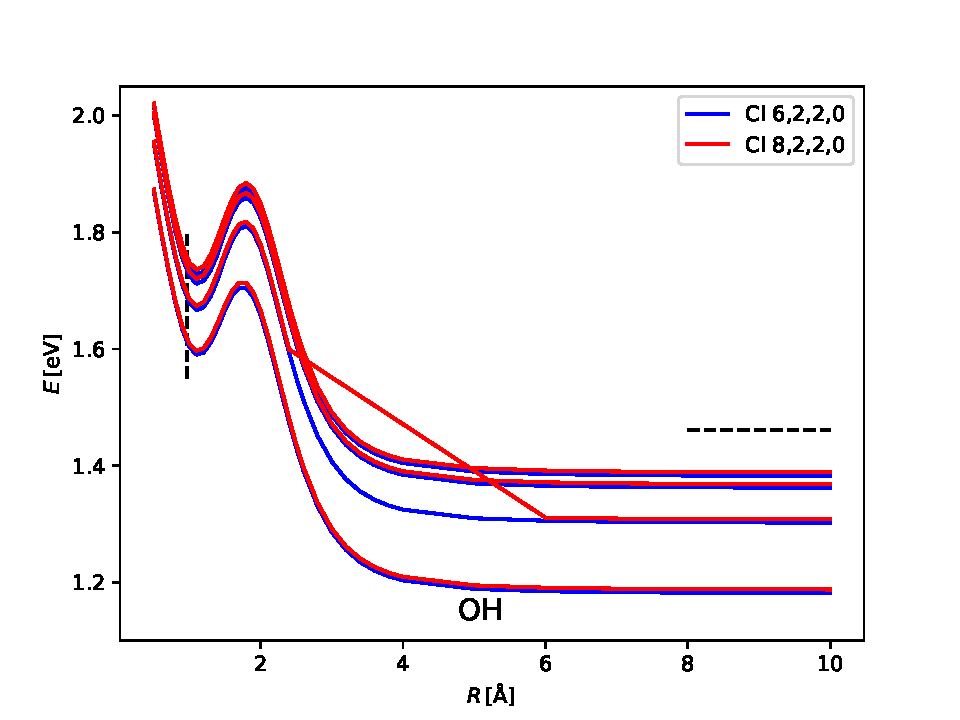
\includegraphics[width=0.95\textwidth]{../img/OH-lin.pdf}
\caption{Rozdíl potenciální křivky neutrální molekuly a aniontu získaných metodami MRCI 
6,2,2,0 a MRCI 8,2,2,0 v bázích aug-cc-pVXZ, $\mathrm{x \in \left\lbrace D,T,Q,5\right
\rbrace }$. vodorovnou přerušovanou čarou je vyznačeno správné asymptotické chování, 
svislou rovnovážná mezijaderná vzdálenost neutrální molekuly.}
\label{grOHlin}
\end{figure}

\begin{figure}
\centering
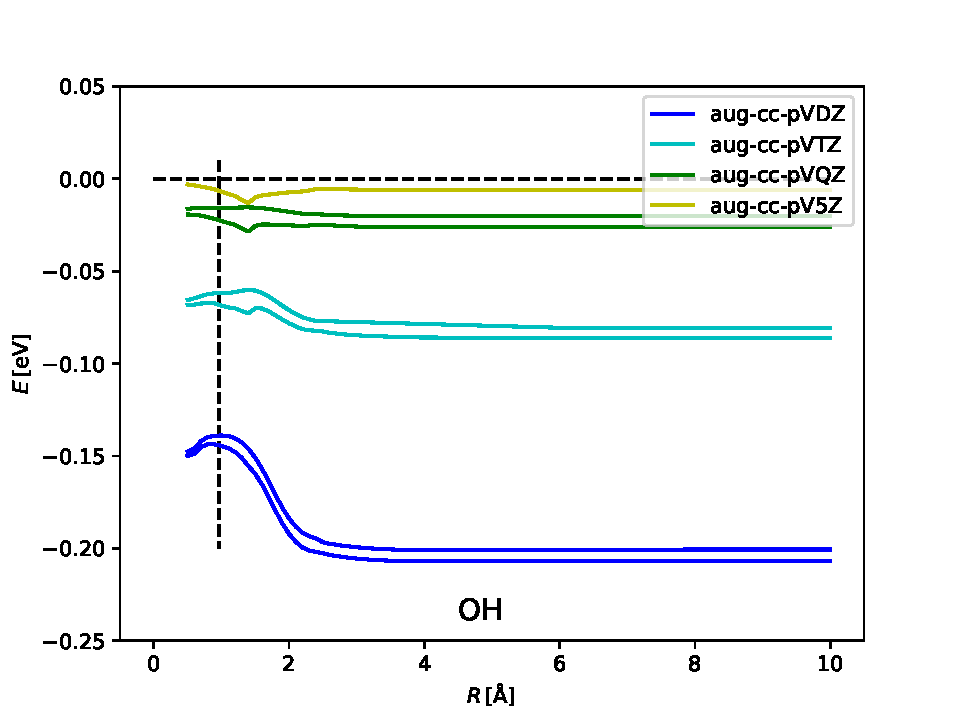
\includegraphics[width=0.95\textwidth]{../img/OH-lin-dif.pdf}
\caption{\TD}
\label{grOHlindif}
\end{figure}

Vibrační energetické hladin pro křivky neutrální molekuly, získané různými metodami 
jsou v tabulce \ref{oh_vibr}. Experimentální hodnoty jsou převzaté z 
\cite{OH_vibr}. Je vidět, že metoda CI 8,2,2,0 v aug-cc-pV5Z bázi  dává hodnoty téměř 
shodné s experimentálními, ale CI 6,2,2,0 ve stejné bázi, nebo extrapolace těchto metod 
nedává příliš velkou odchylku. 
Proto  považujeme za vhodnou metodu pro referenční výpočty MRCI s aktivním prostorem 
pro vstupní CAS-SCF 8,2,2,0 v aug-cc-pV5Z,nebo lépe extrapolované na úplnou bázi, kde 
se shodují disociační energie. Je třeba ale posunou křivky tak, aby se shodovala 
elektronová afinita molekuly s experimentem.

\htable{../tbl/OH-vibr.tex}{Nejnižší čtyři vibrační hladiny molekuly $\mathrm{OH}$ získané pomocí MRCI s různými aktivními prostory vstupního CASSCF a různých bázích.}{oh_vibr}

\subsection{Popis targetu}
Výpočet pomocí R-maticových výpočtů byl na molekule OH proveden a je popsán v 
\cite{OH_Rmatrix}. Zde pro popis targetu použili FCI v omezené množině stavů (CAS-CI), 
tato metoda je podobná metodě CAS-SCF, ale neprobíhá zde optimalizace jednotlivých 
molekulových orbitalů. Aktivní prostor by odpovídal prostoru 4,2,2,0. Výpočty navíc 
prováděli v bázi slaterovského typu, které se dosti liší od gaussovských, které jsme 
používali my. Navíc uvažovali jen jeden excitovaný stav targetu.

Nejprve jsme provedli výpočet křivek pro srovnání metodou MRCI s 
aktivním prostorem pro vstupní CAS-SCF 6,2,2,0 a bází aug-cc-pVQZ. Ten v jednom bodě 
okolo rovnováhy dává špatnou hodnotu, jak je patrno z grafů, ale to není pro srovnání s 
našimi výpočty podstatné. Poté jsme hledali CAS-SCF s vhodným aktivním prostorem.

Ukázalo se, stejně 
jako pro molekulu BeH, že z metod použitelných v rozptylových výpočtech dobře popisuje 
tuto molekulu CAS-SCF v bázi aug-cc-pVDZ s aktivním prostorem $6,2,2,0$. Křivky  
získané touto metodou, spolu s referenčními křivkami v pozadí jsou v grafu 
\ref{gr_OH_6220}. Na rozdíl od výpočtu touto metodou pro molekulu BeH je zde vidět 
nefyzikální nespojitost pro mezijadernou vzdálenost kolem $0.9\AA$. Tu jsme se 
pokusili odstranit nastavením vhodných vah v metodě SA-CASSCF pro různé stavy. K 
odstranění nespojitosti 
vedlo nastavení hodnoty váhy 0.25 na na oba degenerované 
stavy základní křivky $^2\Pi$ ,
váhy 1.0 na nejnižší stav  $^2\Sigma^+$ (Nejnižší vázaný excitovaný stav), 0.5 na 
nejnižší stav  $^2\Sigma^-$ (váha na tomto stavu se ukázala být zásadní pro 
spojitost křivek) a nulovou váhou na všech ostatních stavech. Toto uspořádání vah 
zajistilo spojitost pro všechny námi použité volby aktivního prostoru.

V grafu \ref{gr_OH_7330_w} je pak výpočet pomocí CAS-SCF s vahami podobně 
jako u předchozího zmíněného výpočtu a aktivním prostorem $7,3,3,0$. Ten vykazuje 
nepatrně lepší výsledky pro zmíněný první excitovaný stav, ale za cenu většího 
aktivního prostoru a tím pádem i větší výpočetní náročnosti. Ale u tohoto výpočtu se 
výrazně rozchází asymptotická energie pro stavy jdoucí k prostřední asymptotě, která 
by správně měla být degenerovaná. To značí, že aktivní prostor je nevyvážený, protože 
popisuje některé stavy molekuly lépe než jiné. Ale asymptotické chování není při popisu 
targetu příliš podstatné.

Pro srovnání s výše zmíněným článkem jsme provedli CAS-SCF výpočet s aktivním prostorem 
$4,2,2,0$ v aug-cc-pVDZ bázi. Opět jsme museli použít výše zmíněné váhy.
Výsledek je v grafu \ref{gr_OH_4220_w}. Výsledky se zdají být silně neuspokojivé, je 
špatně popsán i základní stav, který má zjevné jinou rovnovážnou vzdálenost oproti 
referenčnímu výpočtu. Na druhou stranu z toho nelze dělat nějaké závěry kvůli lehce 
odlišné metodě, a úplně jiné použité bázi.

Nakonec jsme provedli výpočet pomocí CAS-SCF s aktivním prostorem 6,2,2,0 v bázích cc-
pVDZ a cc-pVTZ, které jsou v grafu \ref{gr_OH_6220_na}. Z grafu je vidět, že mezi 
popisem v těchto dvou bázích je relativně malý rozdíl. Zároveň ale výpočet stejnou 
metodou  v bázi aug-cc-pVDZ dává o něco lepší výsledky.

Proto za vhodný popis targetu lze považovat SA-CAS-SCF v aug-cc-pVDZ s aktivním 
prostorem 6,2,2,0 nebo 7,3,3,0 s výše popsanými vahami jednotlivých stavů

\begin{figure}
\centering
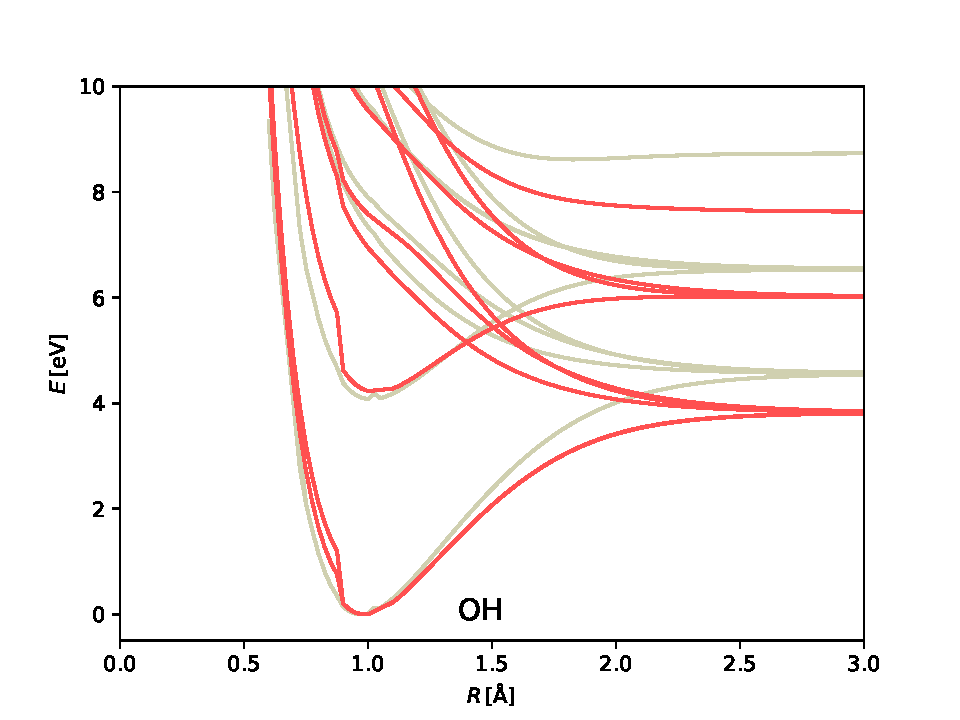
\includegraphics[width=0.95\textwidth]{../img/OH-MULTI-DZ-6220.pdf}
\caption{Srovnání CAS-SCF výpočtu s aktivním prostorem $6,2,2,0$ v aug-cc-pVDZ bázi 
s referenčním MRCI}
\label{gr_OH_6220}
\end{figure}

\begin{figure}
\centering
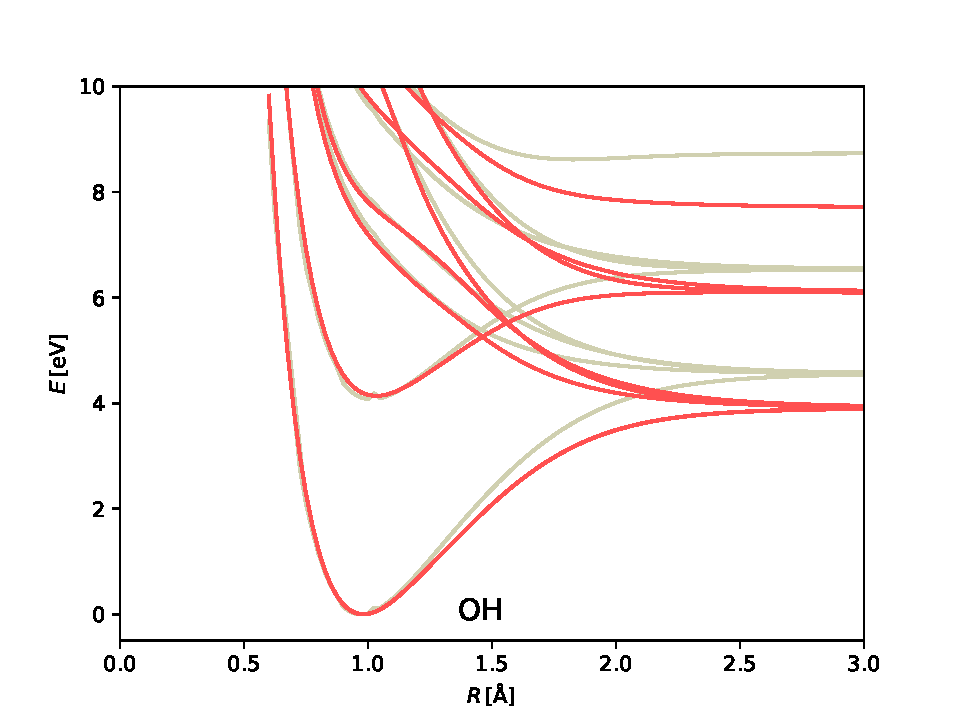
\includegraphics[width=0.95\textwidth]{../img/OH-MULTI-DZ-6220-w8.pdf}
\caption{Srovnání CAS-SCF výpočtu s aktivním prostorem $6,2,2,0$ v aug-cc-pVDZ bázi a upravenými vahami s referenčním MRCI}
\label{gr_OH_6220_w}
\end{figure}

\begin{figure}
\centering
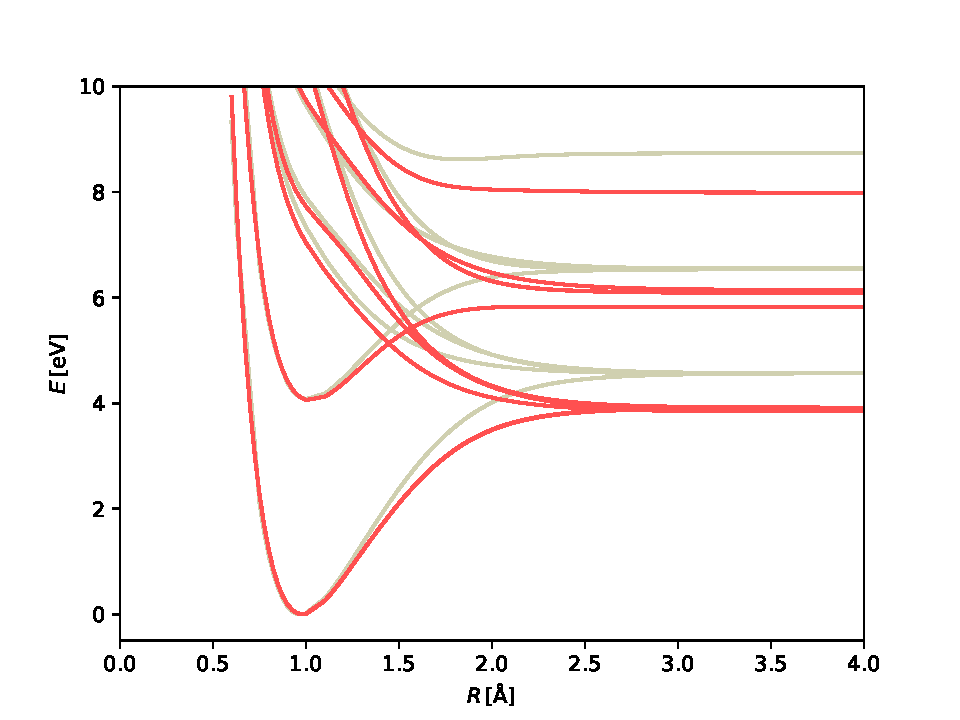
\includegraphics[width=0.95\textwidth]{../img/OH-MULTI-DZ-7330-w1.pdf}
\caption{Srovnání CAS-SCF výpočtu s aktivním prostorem $7,3,3,0$ v aug-cc-pVDZ bázi a upravenými vahami s referenčním MRCI}
\label{gr_OH_7330_w}
\end{figure}

\begin{figure}
\centering
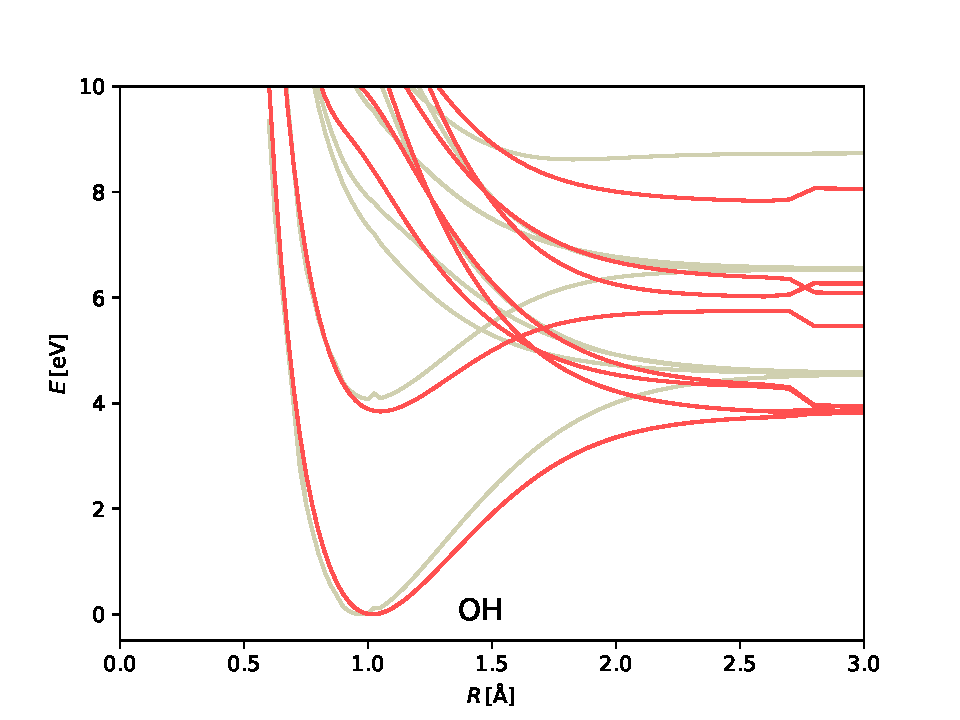
\includegraphics[width=0.95\textwidth]{../img/OH-MULTI-DZ-4220-w1.pdf}
\caption{Srovnání CAS-SCF výpočtu s aktivním prostorem $4,2,2,0$ v aug-cc-pVDZ bázi a  
upravenými vahami s referenčním MRCI}
\label{gr_OH_4220_w}
\end{figure}

\begin{figure}
\centering
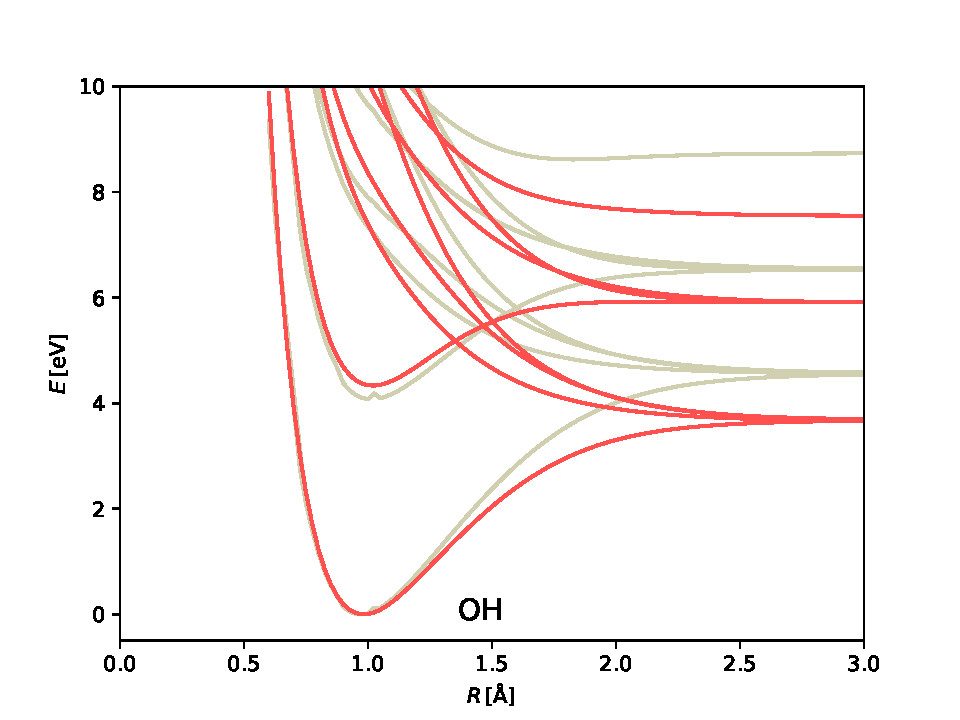
\includegraphics[width=0.95\textwidth]{../img/OH-MULTI-DZna-6220.pdf}
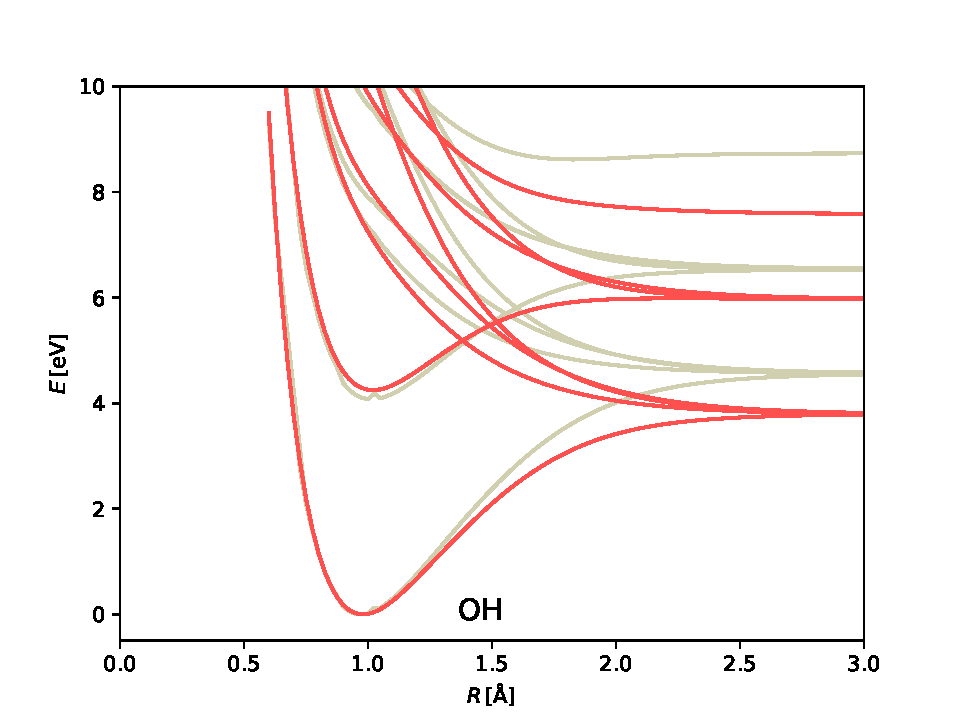
\includegraphics[width=0.95\textwidth]{../img/OH-MULTI-TZ-6220.pdf}
\caption{Srovnání CAS-SCF výpočtu s aktivním prostorem $6,2,2,0$ v cc-pVDZ bázi 
(nahoře) a v cc-pVTZ bázi (dole) s referenčním MRCI}
\label{gr_OH_6220_na}
\end{figure}
